%!TEX root = ../template.tex
%%%%%%%%%%%%%%%%%%%%%%%%%%%%%%%%%%%%%%%%%%%%%%%%%%%%%%%%%%%%%%%%%%%
%% chapter5.tex
%% NOVA thesis document file
%%
%% Chapter 5: Results and Evaluation
%%%%%%%%%%%%%%%%%%%%%%%%%%%%%%%%%%%%%%%%%%%%%%%%%%%%%%%%%%%%%%%%%%%

\typeout{NT FILE chapter5.tex}%

\chapter{Results and Evaluation}
\label{cha:discussion}

This chapter evaluates the computational performance, scalability limits, and runtime feasibility of the proposed \gls{DT} framework. The central premise of this work is that industrial simulation environments can be assembled and executed procedurally from standardized, vendor-neutral \gls{AAS} packages without relying on hard-coded scenes or static configuration files.

The remainder of this chapter is organized as follows:
\begin{itemize}
    \item \Cref{sec:eval_case_study} presents an end-to-end qualitative case study demonstrating how an industrial mechatronic module is authored, packaged into \gls{AAS}, uploaded to the registry, and procedurally instantiated in Unity.
    \item \Cref{sec:eval_fms_bench} provides an empirical validation benchmarking the complete digital replica of the physical modular \gls{FMS} bench across 100 cold-boot execution lifecycles.
    \item \cref{sec:eval_stress_testing} conducts a parametric scalability stress test evaluating computational boundaries across eight scale levels ($N \in \{5, \dots, 1000\}$ conveyor modules).
    \item \Cref{sec:eval_discussion} synthesizes practical findings, discusses computational limitations and geometric trade-offs, and systematically verifies the research hypotheses.
\end{itemize}

All benchmark tests were executed on a Lenovo laptop equipped with a 13th Generation Intel Core i7-13650HX processor (14 cores, 20 threads up to 4.9\,GHz), 16\,GB of DDR5 \gls{RAM}, and an NVIDIA GeForce RTX 4060 Laptop \gls{GPU} with 8\,GB of \gls{VRAM}, running Windows 11 Home (version 25H2) and Unity 6 (version 6000.3.10f1).

% =============================================================================
% SECTION: QUALITATIVE DEMONSTRATOR / ONBOARDING WALKTHROUGH
% =============================================================================

\section{Demonstrative Case Study: End-to-End Asset Onboarding}
\label{sec:eval_case_study}

To validate the practical usability and operational workflow of the framework (addressing the visual modeling objective and requirement \textbf{NFR4}), this section presents an end-to-end walkthrough demonstrating the onboarding of a new mechatronic asset: introducing an additional modular conveyor unit, designated as \textbf{Conveyor~G} (Asset ID: \texttt{Conveyor\_G}), into the production line. The case study demonstrates how this new equipment is designed, semantically enriched, packaged into a standardized \gls{AAS}, and procedurally executed as an active \gls{DT} without modifying or recompiling the simulation scene.

The onboarding lifecycle spans five sequential stages, progressing from initial 3D mesh modeling to operational \gls{DT} execution:

\subsection{\texorpdfstring{\gls{CAD}}{CAD} Design and Kinematic Rigging in Blender}
To guarantee full geometric control, lightweight rendering, and accurate dimensional conformity with the physical equipment, mechatronic modules are designed directly from scratch in Blender rather than relying on unoptimized third-party exports. As described in \Cref{sec:impl_layer0} and illustrated in \Cref{fig:fms_physical_vs_blender} (\cpageref{fig:fms_physical_vs_blender}), the mechanical structure is modeled to scale based on physical tape measurements of the testbed. 

The mesh reproduces the functional geometry while avoiding redundant internal features, ensuring high real-time rendering efficiency. The assembly is partitioned into distinct sub-meshes separating static frame elements from mobile components, such as conveyor belts. The local coordinate origin (\textit{pivot point}) of each mobile part is positioned on its physical axis of motion (rotational center for rotating conveyors or linear axis for translation), preventing geometric distortion during procedural runtime animations. Finally, the finished assembly is exported as a single binary \gls{GLB} container with embedded materials and standard $Y$-up coordinate orientation.

\subsection{3D Model Ingestion and Hierarchy Verification}
With the \gls{GLB} file produced, the automation engineer opens the lightweight Asset Modeling Desktop Application (\Cref{sec:impl_wizard}). As demonstrated in \Cref{fig:conveyor_wizard_gui_screenshot} (\cpageref{fig:conveyor_wizard_gui_screenshot}), the application provides an interactive 3D viewport powered by an embedded rendering engine. 

The engineer loads the binary \gls{GLB} file into the workspace, prompting the ingestion pipeline to parse the internal scene graph, normalize bounding dimensions, and populate the interactive node hierarchy tree. The user inspects the component to verify that node names match the intended physical taxonomy and confirms that pivot orientations align with expected motion vectors before proceeding to semantic pin configuration.

\subsection{Interactive Pin Mapping and Control Logic Definition}
In the third stage, the engineer equips the geometric mesh with cyber-physical semantics without writing software scripts. Rather than manually measuring and typing three-dimensional coordinates, the engineer clicks directly onto the surface of the conveyor mesh in the viewport. The application casts a ray from the camera, calculates the exact surface intersection point, and computes the surface normal vector.

A virtual optical beam sensor is aligned along the surface normal and anchored to the clicked coordinate. In the configuration panel, the user specifies its operational properties, including register binding (\texttt{I0\_0}), polarity (active-low), and ground-truth workpiece snapping coordinates for position drift correction. Moving parts, such as the conveyor surface, are bound to actuator registers (\texttt{R0\_2}). If local edge behavior is needed, such as stopping the belt automatically when a photoeye is blocked without waiting for master \gls{PLC} polling, the user defines local event-condition-action rules in the \textit{ControlLogic} editor.

\begin{figure}[htbp]
    \centering
    \begin{subfigure}[b]{0.95\linewidth}
        \centering
        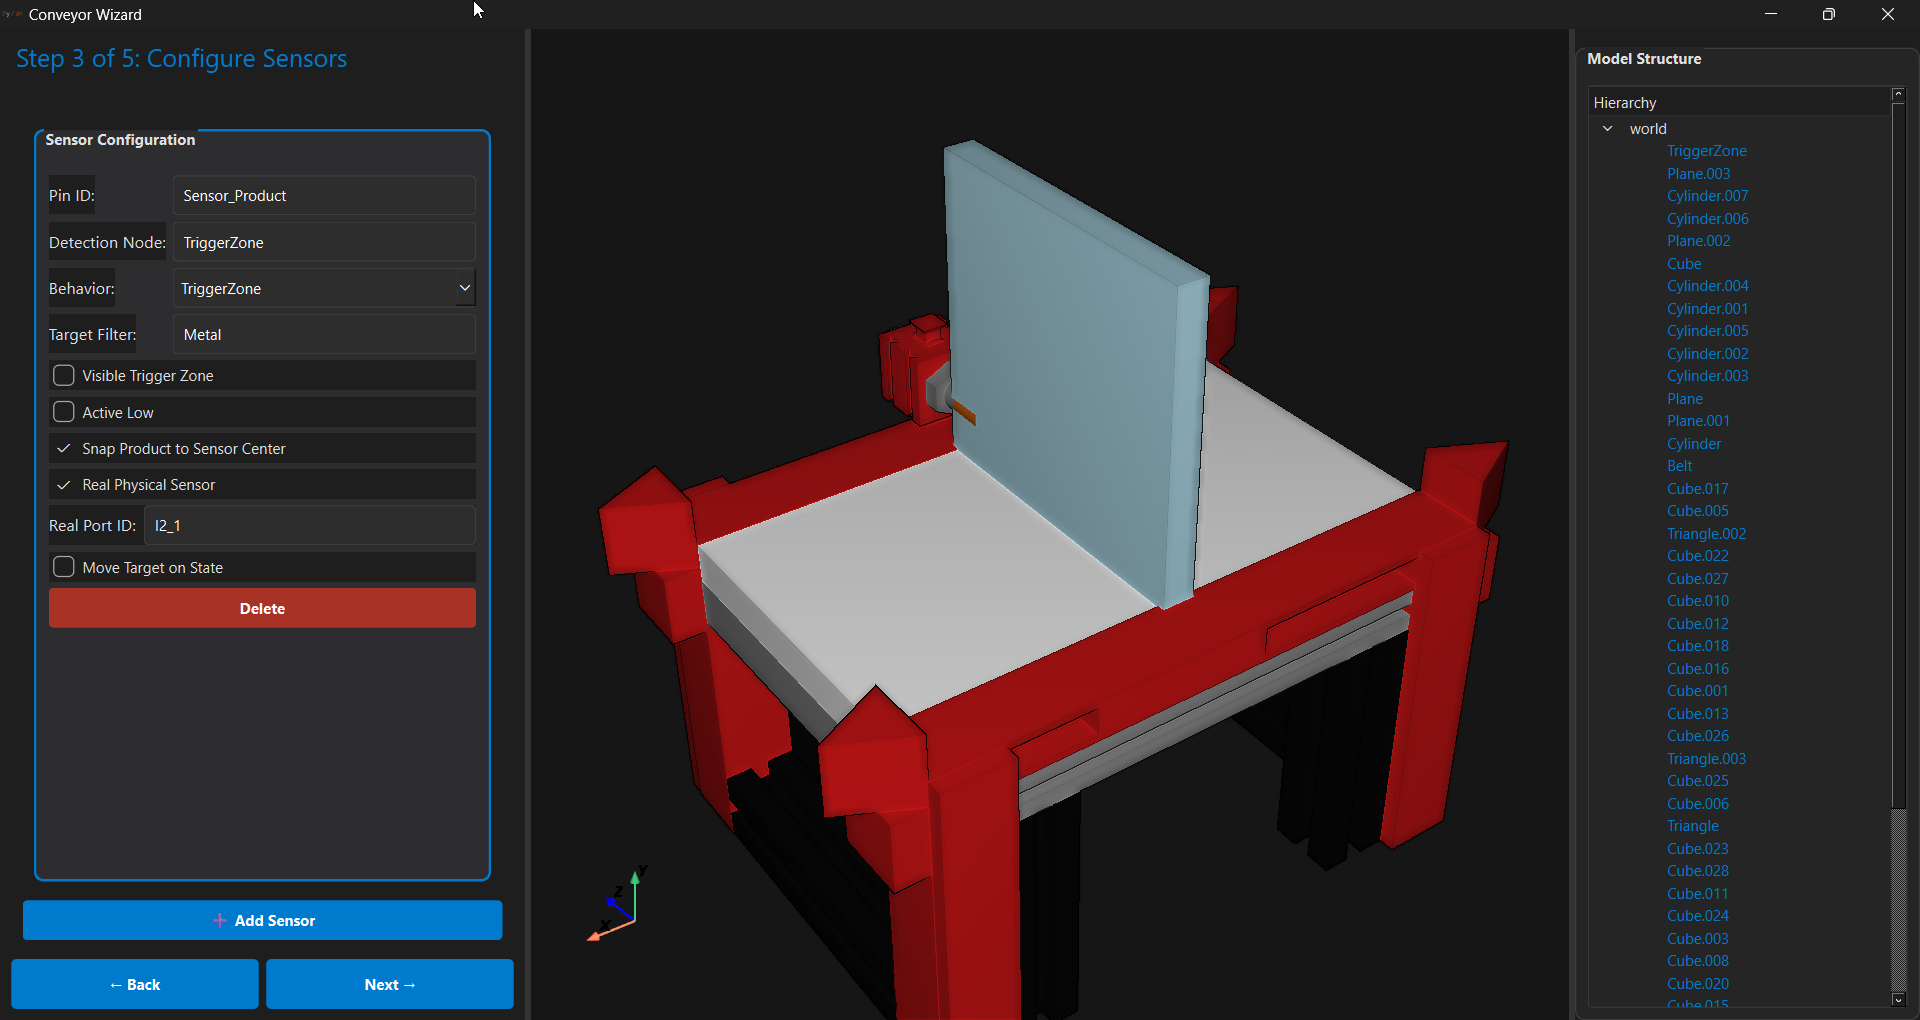
\includegraphics[width=\linewidth,height=0.34\textheight,keepaspectratio]{5-Figures/5-sensores}
        \caption{Interactive optical sensor placement via surface raycasting.}
        \label{fig:case_study_step2_sensors}
    \end{subfigure}
    \par\vspace{0.4cm}
    \begin{subfigure}[b]{0.95\linewidth}
        \centering
        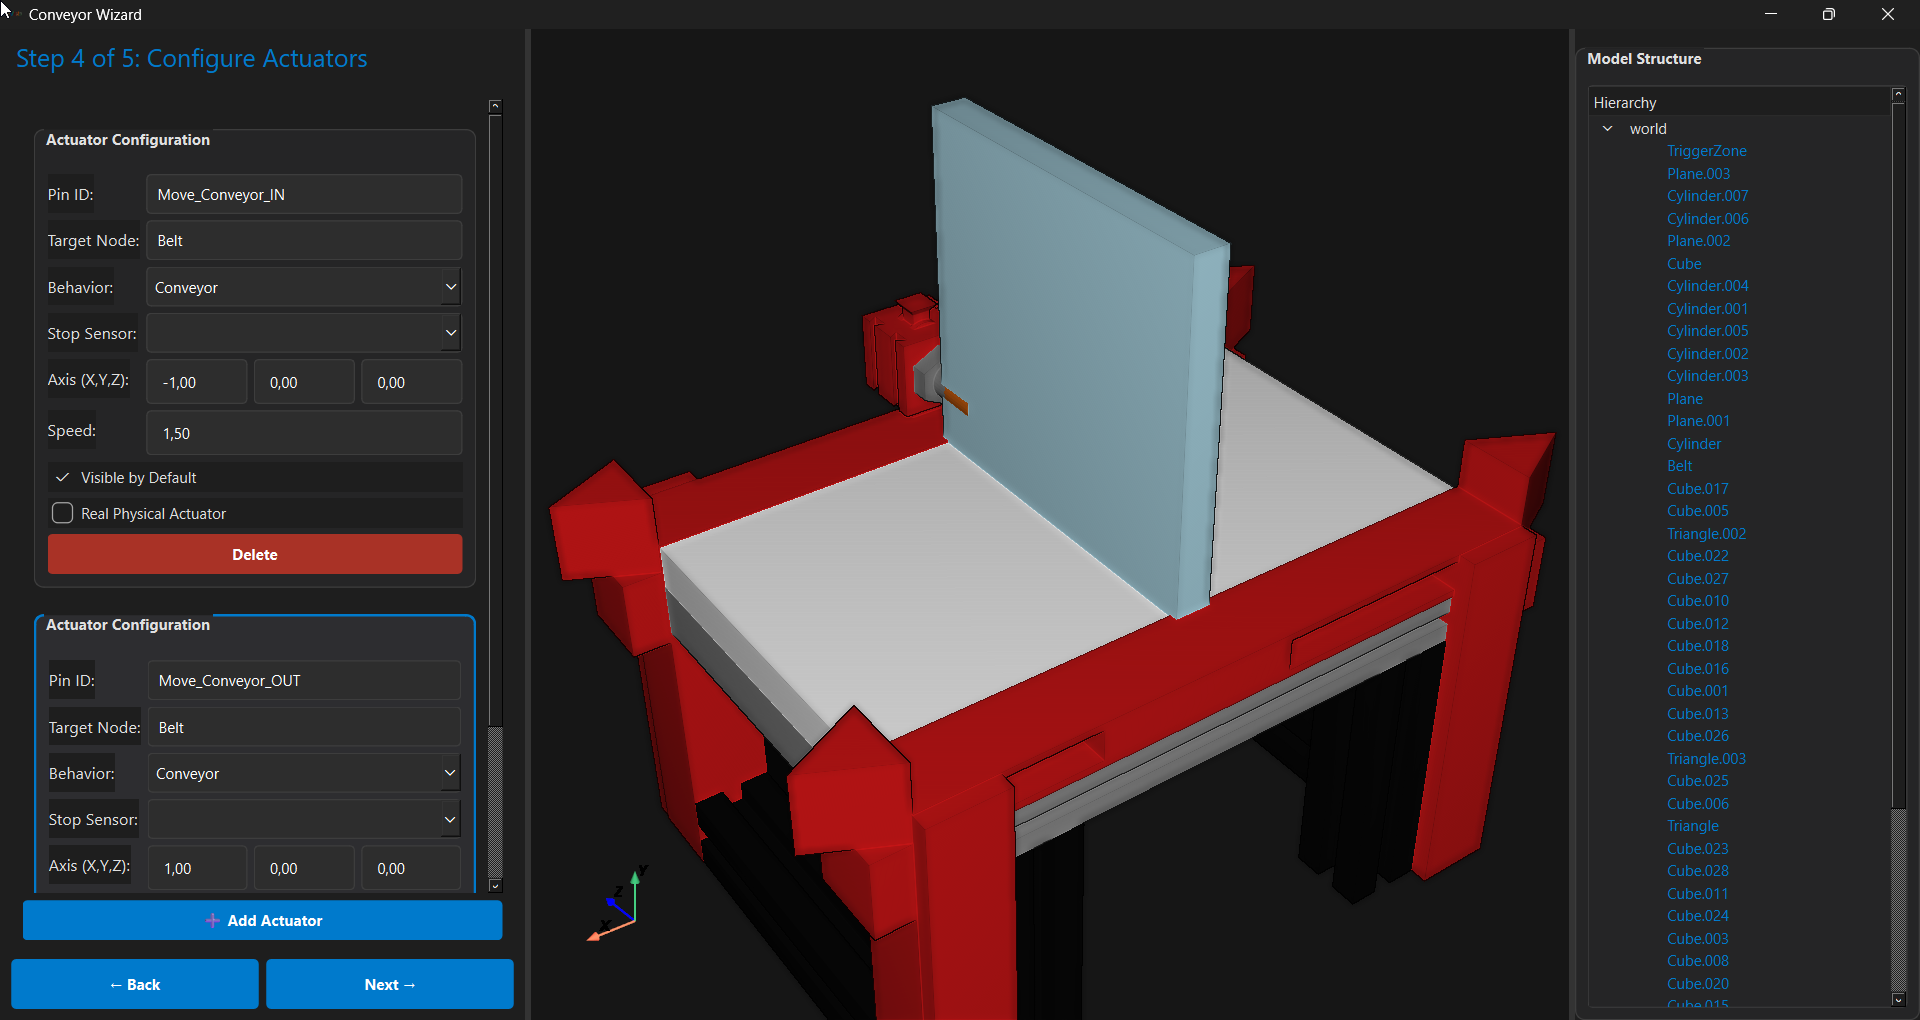
\includegraphics[width=\linewidth,height=0.34\textheight,keepaspectratio]{5-Figures/5-atuadores}
        \caption{Actuator kinematic configuration and output register binding.}
        \label{fig:case_study_step2_actuators}
    \end{subfigure}
    \caption{Interactive virtual pin mapping in the desktop onboarding wizard, showing: (a) sensor placement using surface raycasting, and (b) kinematic actuator binding.}
    \label{fig:case_study_step2}
\end{figure}

\subsection{Control Logic Rule Definition}
Following signal and kinematic configuration, the engineer specifies autonomous edge behavior for Conveyor~G using the visual Rule Editor introduced in \Cref{fig:rule_editor_ui} (\cpageref{fig:rule_editor_ui}). Rather than writing low-level code or proprietary scripts, the engineer composes event-condition-action statements through visual blocks. For this conveyor module, a transfer sequence named \textit{A$\rightarrow$G} is defined: belt motion starts when the sensor on Conveyor~A is triggered and stops once the sensor on Conveyor~G is activated. These rules are serialized into the standard \textit{ControlLogic} submodel schema, allowing the runtime to execute localized automation independently of external supervisory intervention.

\subsection{\texorpdfstring{\gls{AASX}}{AASX} Compilation and Repository Publication}
Once physical geometry, pin assignments, behavioral bindings, and operational rules are defined, the engineer triggers package export. The tool uses the Eclipse BaSyx Python \gls{SDK} to generate the standardized submodel descriptors that describe the asset: \textit{VisualStructure} (mesh references, node hierarchy, and spatial transforms), \textit{VirtualPins} (input and output signal interfaces), \textit{BehaviorMapping} (kinematic parameters, speeds, motion vectors, and sensing trigger envelopes), \textit{AssetInterfacesDescription} (network communication endpoints and protocol bindings), and optionally \textit{ControlLogic} (autonomous edge rules for virtual commissioning).

The serialized submodel definitions and the binary \gls{GLB} mesh are packed into an \gls{OPC} \gls{AASX} container file. The application dispatches an \gls{HTTP} POST request directly to the centralized Eclipse BaSyx v2 server. As shown in the BaSyx AAS Viewer in \Cref{fig:case_study_step3}, the server unpacks the container, exposes the submodels through standard \gls{REST} endpoints, and registers the global Asset ID in the \gls{AAS} Registry.

\begin{figure}[htbp]
    \centering
    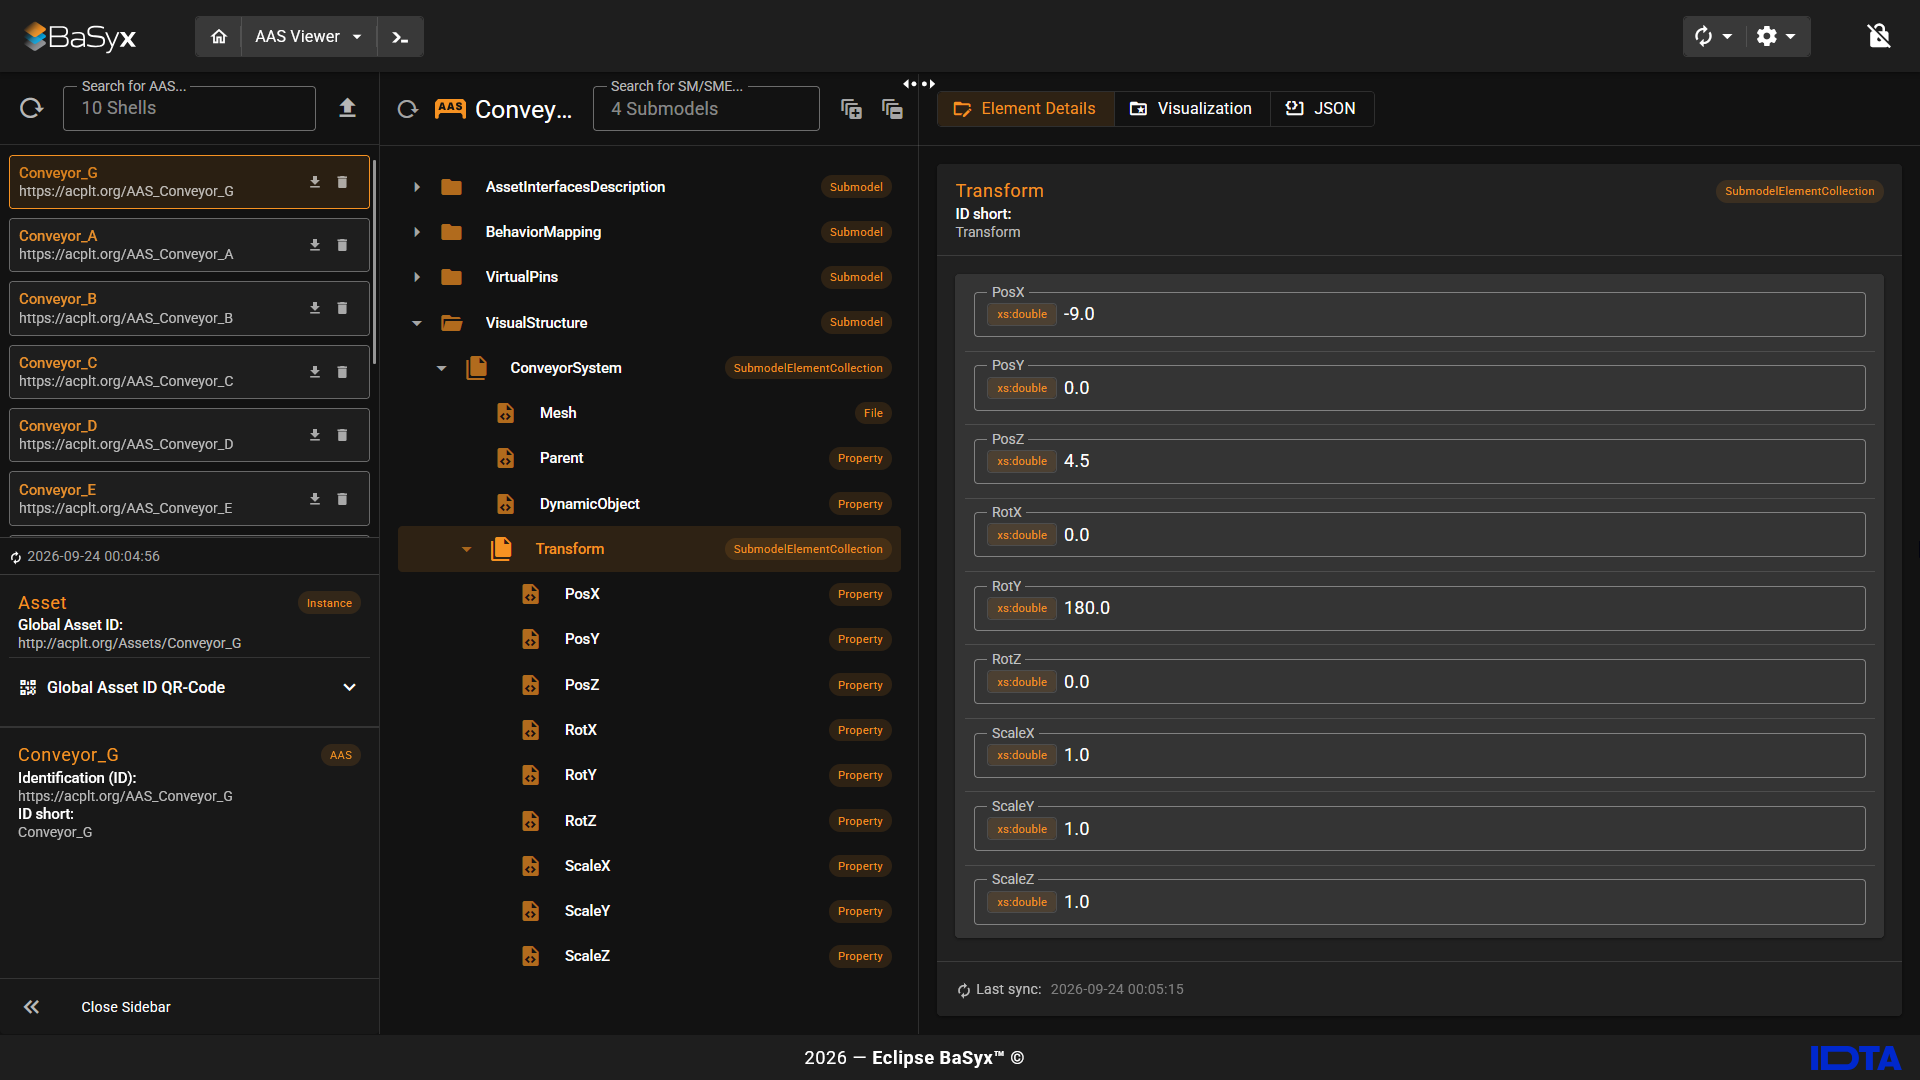
\includegraphics[width=0.90\linewidth,height=0.38\textheight,keepaspectratio]{5-Figures/5-aas}
    \caption{Standardized \gls{AASX} container for Conveyor~G uploaded and registered in the Eclipse BaSyx v2 repository, displaying its submodels in the AAS Viewer.}
    \label{fig:case_study_step3}
\end{figure}

\subsection{Zero-Touch Procedural Instantiation and Live Telemetry}
In the final stage, the Unity 3D simulation environment is launched without pre-baked assets. Upon initialization, the Unity runtime queries the BaSyx registry over \gls{REST}, retrieves active Asset IDs, and downloads the associated \gls{GLB} binary files and submodel manifests into transient memory.

The runtime procedural builder parses the \textit{VisualStructure} and instantiates the mesh hierarchy, inspecting component meshes dynamically to attach optimized physics colliders and configure physical rigidbodies. The builder then parses \textit{VirtualPins} and \textit{BehaviorMapping} to instantiate trigger zones at the exact coordinates recorded during raycasting, binding them to internal signal dispatchers, while configuring surface velocities, rotation axes, and constraints onto designated mobile parts. If present, \textit{ControlLogic} rules are loaded by the local rule interpreter, completing the procedural assembly of the simulation scene (\Cref{fig:case_study_step4}).

Finally, the simulation engine connects to the physical controller via \gls{TCP} telemetry. When a workpiece on the physical workbench crosses an optical sensor, the physical \gls{PLC} sets register \texttt{I0\_0} to HIGH. The telemetry listener receives the frame, trips the corresponding virtual sensor indicator, and immediately executes kinematic position snapping to reconcile any cumulative micro-slip, maintaining sub-millimeter positional fidelity throughout production cycles.

\begin{figure}[htbp]
    \centering
    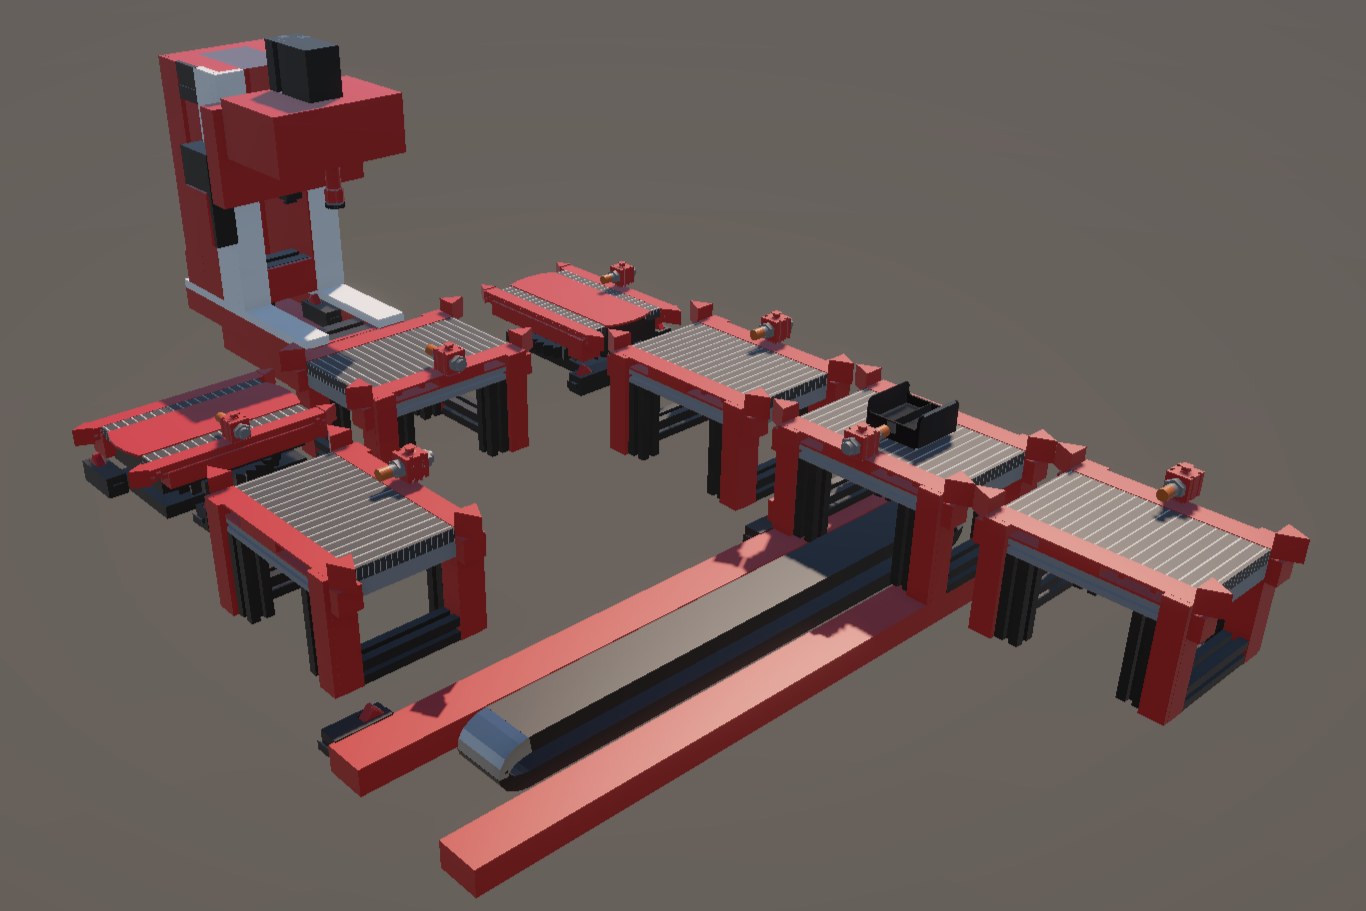
\includegraphics[width=0.90\linewidth,height=0.38\textheight,keepaspectratio]{5-Figures/5-unity}
    \caption{Procedural scene assembly and operational \gls{DT} execution in Unity 3D, showing Conveyor~G integrated into the reconstituted simulation scene.}
    \label{fig:case_study_step4}
\end{figure}

% =============================================================================
% SECTION: FMS BENCHMARK
% =============================================================================
\section{Empirical Validation: Modular \texorpdfstring{\gls{FMS}}{FMS} Pilot Bench}
\label{sec:eval_fms_bench}

To validate whether the \gls{DT} operates with sufficient fidelity and responsiveness for physical automation systems, an individual benchmark was dedicated entirely to the modular \gls{FMS} pilot system. Mechanically and functionally, the virtual replica instantiates the exact components of the physical workbench: three linear conveyors, two curved rotational conveyors, one translating conveyor, and the punch station, accompanied by all associated virtual sensing colliders and actuator endpoints.

To evaluate whether the runtime operates with sufficient responsiveness and determinism for industrial automation, several complementary metrics are monitored:
\begin{itemize}
    \item \textbf{Rendering Throughput (\gls{FPS}) and Target Thresholds:} In interactive 3D simulations, 60\,\gls{FPS} (16.6\,ms per frame) is widely regarded as the target benchmark for fluid, real-time visualization and synchronized interaction. A threshold of 30\,\gls{FPS} (33.3\,ms per frame) represents the acceptable operational minimum, below which visual stutter becomes noticeable and input latency can interfere with monitoring.
    \item \textbf{Mean Frame Time:} While \gls{FPS} measures frequency, the frame time (in milliseconds) directly quantifies the computational cost spent by the engine in each update tick, measuring how much margin remains before missing the next frame deadline.
    \item \textbf{1\% Low \gls{FPS}:} The average frame rate of the slowest 1\% of frames. Unlike the overall average \gls{FPS}, which can hide momentary freezing, this metric reveals transient stutter caused by simultaneous sensor triggers or complex collision bursts.
    \item \textbf{P95 and P99 Tail Latency:} The 95th and 99th percentiles of frame render times. In real-time \gls{DT} synchronization, these tail metrics ensure that even rare latency spikes do not breach controller communication windows or cause packet processing delays.
\end{itemize}

An automated test harness conducted 100 independent cold executions of the complete \gls{FMS} cell. In each cycle, the Unity runtime ingested the \gls{AASX} packages, rigged kinematic joints and surface friction physics, linked sensor callbacks, and executed the simulation. \Cref{tab:fms_results} summarizes the performance metrics observed across the 100 test runs.

\begin{table}[htbp]
    \centering
    \caption{Experimental results for the modular \gls{FMS} pilot bench across 100 test runs.}
    \label{tab:fms_results}
    \renewcommand{\arraystretch}{1.3}
    \small
    \begin{tabular}{lrrr}
        \toprule
        \textbf{Metric} & \textbf{Mean $\pm$ Std} & \textbf{Min} & \textbf{Max} \\
        \midrule
        Startup Initialization Time (s)     & $2.79 \pm 0.04$   & $2.72$   & $2.96$   \\
        Steady-State Frame Rate (\gls{FPS}) & $489.91 \pm 49.21$ & $352.66$ & $694.09$ \\
        1\% Low Frame Rate (\gls{FPS})      & $272.43 \pm 87.32$ & $104.60$ & $414.18$ \\
        Mean Frame Time (ms)                & $2.36 \pm 0.39$   & $1.56$   & $3.91$   \\
        P95 Tail Latency (ms)               & $3.84 \pm 1.47$   & $2.38$   & $8.53$   \\
        P99 Tail Latency (ms)               & $4.35 \pm 2.01$   & $2.41$   & $9.94$   \\
        \bottomrule
    \end{tabular}
\end{table}

As shown in \Cref{tab:fms_results}, procedural reconstitution of the pilot bench requires an average of only $2.79\,$s ($\sigma = 0.04\,$s), demonstrating high determinism and repeatability across cold boots. Once initialized, the physics simulation runs at an average of $489.91\,$\gls{FPS}, corresponding to a frame render latency of $2.36\,$ms. Even under transient workpiece transfer loads, the 1\% low frame rate remains at $272.43\,$\gls{FPS}, safely above standard interactive visualization rates.

\Cref{fig:fms_distributions} illustrates the statistical dispersion of these metrics. The startup time exhibits a narrow interquartile range ($2.76\,$s to $2.80\,$s), confirming that semantic archive decompression and mesh generation do not suffer from filesystem blocking. In addition, the rendering rate remains stable around $490\,$\gls{FPS}, exceeding real-time requirements, while the 99th percentile (P99) tail latency stays below $9.94\,$ms across all test runs (\Cref{tab:fms_results}).

\begin{figure}[htbp]
    \centering
    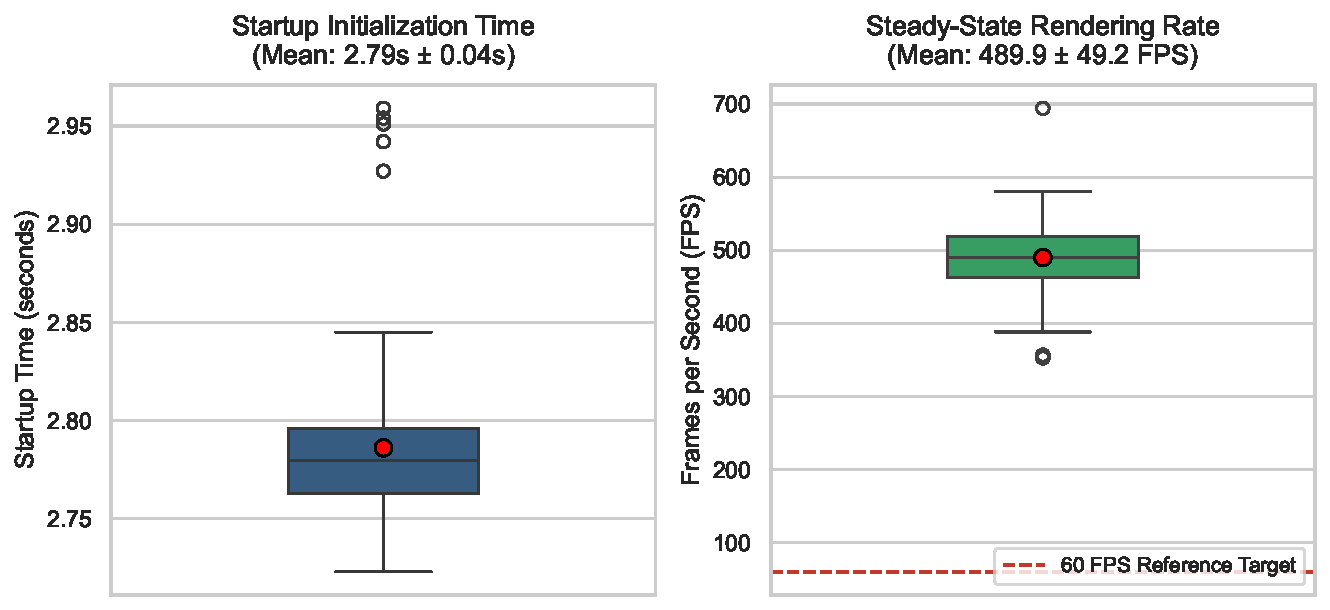
\includegraphics[width=0.88\linewidth,height=0.32\textheight,keepaspectratio]{5-Figures/fms_metrics_distributions.pdf}
    \caption{Distribution of startup initialization time and steady-state rendering frame rate across 100 experimental runs of the modular \gls{FMS} pilot bench.}
    \label{fig:fms_distributions}
\end{figure}

\Cref{fig:fms_timeseries} plots the temporal execution profile during runtime. During the startup window ($t < 2.79\,$s), frame times show transient fluctuations while colliders and textures are bound. As soon as procedural initialization concludes, the system immediately transitions into a flat steady state, confirming that the \gls{DT} operates without frame pacing stutter or cumulative jitter during pallet routing.

\begin{figure}[htbp]
    \centering
    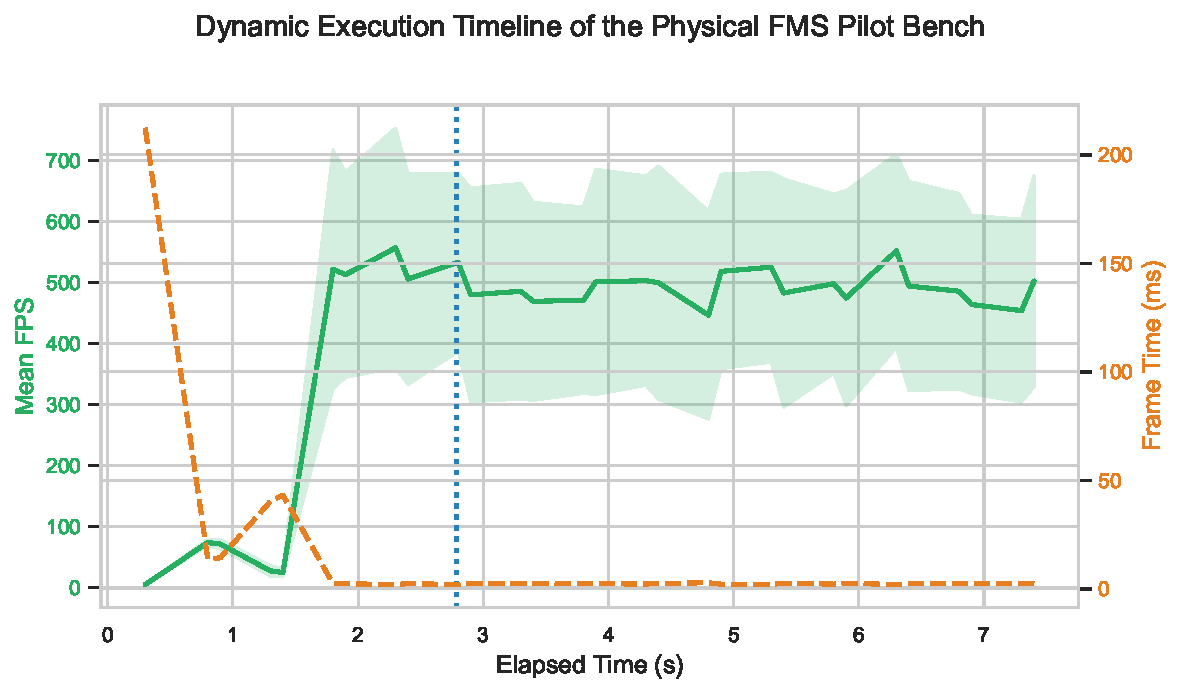
\includegraphics[width=0.88\linewidth,height=0.35\textheight,keepaspectratio]{5-Figures/fms_timeseries_evolution.pdf}
    \caption{Dynamic execution timeline of the modular \gls{FMS} bench, contrasting frame rate with frame latency over simulation time.}
    \label{fig:fms_timeseries}
\end{figure}

% =============================================================================
% SECTION: SCALABILITY AND STRESS BENCHMARK
% =============================================================================
\section{High-Density Scalability Stress Testing}
\label{sec:eval_stress_testing}

While the individual \gls{FMS} benchmark validates operational effectiveness for typical production cells, smart manufacturing facilities often integrate tens or hundreds of interconnected transport segments. To identify the computational ceilings of the pipeline, a parametric stress benchmark was conducted across eight discrete module density levels:
\begin{equation*}
    N \in \{5,\, 10,\, 25,\, 50,\, 100,\, 250,\, 500,\, 1000\} \text{ conveyor modules}.
\end{equation*}

\subsection{Benchmark Methodology and Experimental Test Rig}
\label{sec:eval_methodology}

In this setup, each module represents a complete modular asset encapsulated in an official \gls{AAS} archive (\gls{AASX} format), containing visual meshes (\gls{GLB}), kinematic joints, virtual sensor pins, and behavioral logic. To replicate realistic distributed processing stations, one punch stamping station is procedurally instantiated for every five conveyor modules, placed at module index~3 and subsequently every 5 modules ($i \in \{3,\, 8,\, 13,\, 18,\, \dots\}$). At $N=5$, 5 conveyors and 1 punch mechanism are instantiated (\Cref{fig:eval_benchmark_setup}), scaling up to 1000 conveyors and 200 punch stations at $N=1000$.

\begin{figure}[htbp]
    \centering
    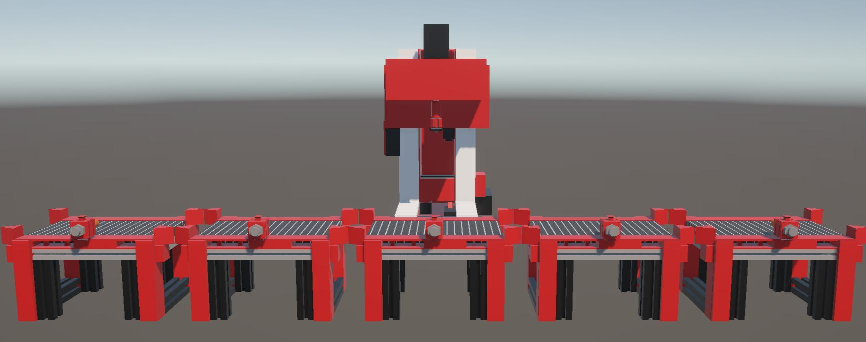
\includegraphics[width=0.90\linewidth,height=0.35\textheight,keepaspectratio]{5-Figures/teste_5_conveyors.pdf}
    \caption{Procedural benchmark simulation layout showcasing the modular arrangement of conveyors and integrated punch stations (1 punch mechanism per 5 conveyors).}
    \label{fig:eval_benchmark_setup}
\end{figure}

For each scale level $N$, 100 independent automated runs were executed, recording metrics at 500\,ms intervals over a steady-state execution window (totaling 800 simulation lifecycles). \Cref{tab:consolidated_results} summarizes the consolidated results. Note that at the highest density ($N=1000$), the large standard deviation in frame rate reflects heavy distribution skewness caused by brief transient bursts interspersed between severe physics bottlenecks, rather than a symmetric Gaussian distribution.

\begin{table}[htbp]
    \centering
    \caption{Consolidated stress test results across 800 benchmark runs (Mean $\pm$ Standard Deviation).}
    \label{tab:consolidated_results}
    \renewcommand{\arraystretch}{1.3}
    \small
    \begin{tabular}{rrrr}
        \toprule
        \textbf{Conveyors} & \textbf{Startup Time (s)} & \textbf{Mean \gls{FPS}} & \textbf{Frame Time (ms)} \\
        \midrule
        5    & $2.61 \pm 0.10$    & $460.80 \pm 63.73$ & $2.49 \pm 0.27$    \\
        10   & $2.85 \pm 0.04$    & $418.03 \pm 52.84$ & $2.69 \pm 0.28$    \\
        25   & $3.66 \pm 0.05$    & $369.42 \pm 52.10$ & $3.10 \pm 0.36$    \\
        50   & $5.22 \pm 0.09$    & $344.68 \pm 46.22$ & $3.30 \pm 0.37$    \\
        100  & $8.55 \pm 0.11$    & $313.00 \pm 51.02$ & $3.73 \pm 0.51$    \\
        250  & $20.60 \pm 0.40$   & $254.24 \pm 45.37$ & $5.43 \pm 1.42$    \\
        500  & $57.45 \pm 2.77$   & $93.16 \pm 20.98$  & $14.96 \pm 4.68$   \\
        1000 & $416.70 \pm 135.08$& $13.96 \pm 43.28$  & $342.21 \pm 110.59$\\
        \bottomrule
    \end{tabular}
\end{table}

\subsection{Startup Initialization and Procedural Instantiation Complexity}
\label{sec:eval_startup_complexity}

A critical measure of practical usability is the time required for the virtual runtime to discover, parse, and instantiate an arbitrary factory line. \Cref{fig:eval_startup_complexity} displays the scaling trend of the total startup initialization time alongside the unit instantiation cost per module across all scale levels ($N \in \{5, \dots, 1000\}$).

The empirical results show that for realistic production line scales (between 5 and 50 conveyors), the procedural generation process is nearly instantaneous. Initializing a cell of 5 conveyors required an average of $2.61\,$s ($\sigma = 0.10\,$s), while a 50-conveyor installation initialized in $5.22\,$s ($\sigma = 0.09\,$s). Scaling to a facility of 100 conveyors took $8.55\,$s ($\sigma = 0.11\,$s), and a large 250-conveyor layout was assembled in $20.60\,$s ($\sigma = 0.40\,$s).

\begin{figure}[htbp]
    \centering
    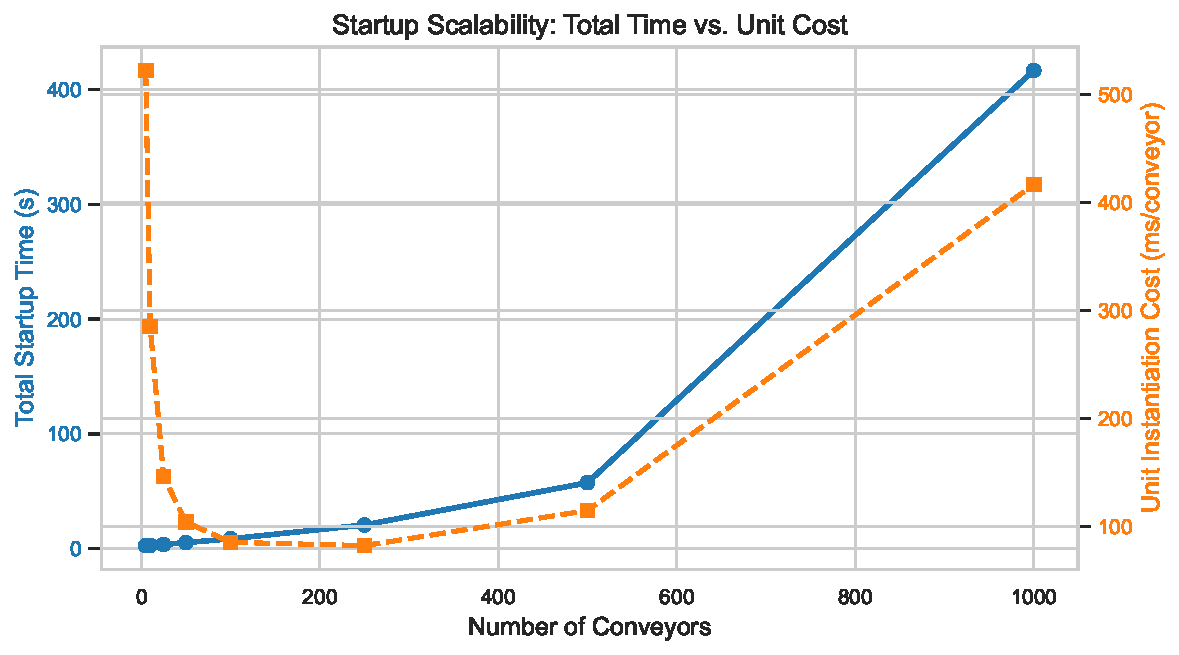
\includegraphics[width=0.88\linewidth,height=0.40\textheight,keepaspectratio]{5-Figures/eval_startup_complexity.pdf}
    \caption{Procedural scaling complexity: total startup initialization time versus unit instantiation cost per conveyor module.}
    \label{fig:eval_startup_complexity}
\end{figure}

As shown in \Cref{fig:eval_startup_complexity}, the unit startup time per conveyor module exhibits an initial downward curve, dropping from 522.0\,ms/module at $N=5$ to 104.4\,ms/module at $N=50$, and reaching a minimum of 82.4\,ms/module at $N=250$. This higher unit time at smaller scales occurs because the Unity engine itself incurs an intrinsic baseline startup latency to bootstrap the core runtime, compile and link dynamic scripts, initialize graphics rendering pipelines, load shader variants, and allocate disk buffers. When only a small number of conveyors is instantiated (such as $N=5$), this substantial fixed engine initialization cost is divided among very few assets, resulting in artificially high unit costs. As the facility scales up to 50 and 250 conveyors, this upfront static engine overhead becomes negligible, amortizing smoothly across the larger asset population until true per-module instantiation complexity dominates.

However, beyond $N=500$, initialization time increases non-linearly, reaching $57.45\,$s at 500 modules and $416.70\,$s at 1000 modules. This escalation is driven by the main-thread bottleneck of Unity's mesh collider generation and the sequential file decompression of multiple \gls{AASX} zip archives.

\subsection{Rendering Fluidity and Frame Rate Degradation}
\label{sec:eval_fluidity_fps}

To evaluate visual responsiveness and stability, \Cref{fig:eval_fps_degradation} illustrates the degradation of mean frame rate alongside the 1\% low frame rate metric (which highlights severe transient frame drops) relative to the industrial 60\,\gls{FPS} target (16.6\,ms) and the 30\,\gls{FPS} critical threshold (33.3\,ms).

\begin{figure}[htbp]
    \centering
    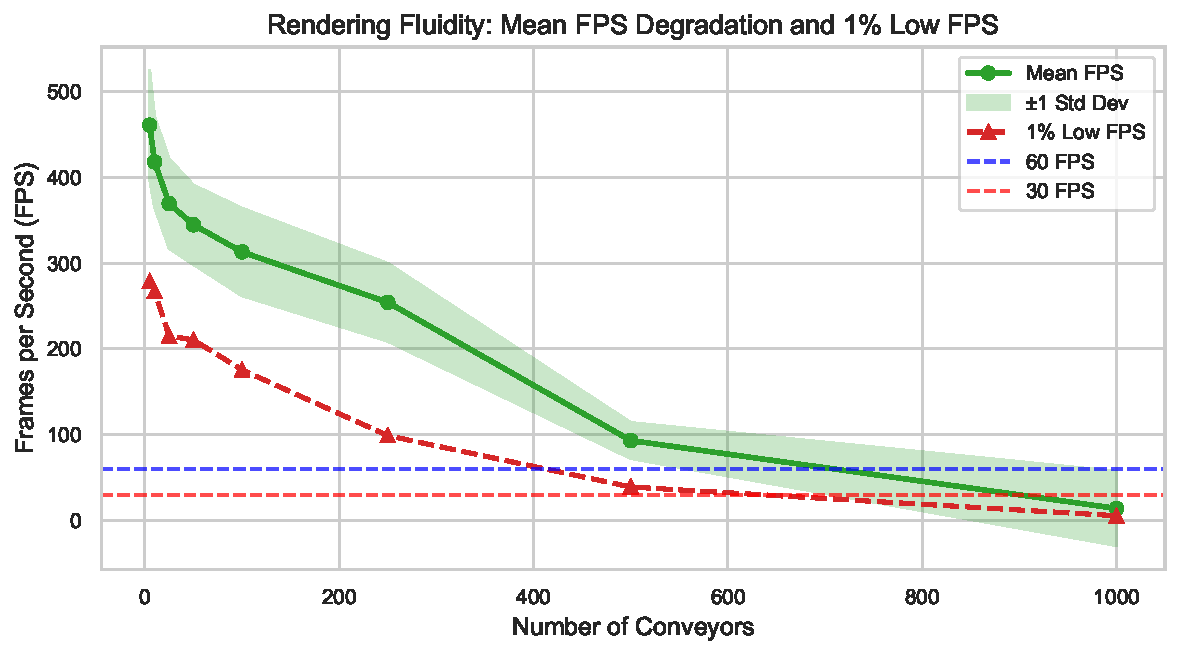
\includegraphics[width=0.88\linewidth,height=0.42\textheight,keepaspectratio]{5-Figures/eval_fps_degradation.pdf}
    \caption{Rendering fluidity and frame rate degradation across conveyor module counts, showing mean steady-state \gls{FPS}, standard deviation, and 1\% low \gls{FPS}.}
    \label{fig:eval_fps_degradation}
\end{figure}

For layouts up to 250 conveyor modules, the procedural \gls{DT} operates with substantial performance headroom. The mean frame rate reaches $460.80\,$\gls{FPS} for 5 conveyors, $344.68\,$\gls{FPS} for 50 conveyors, and $254.24\,$\gls{FPS} for 250 conveyors. The 1\% low frame rate remains above $98.4\,$\gls{FPS} across these scales, confirming that the simulation runs smoothly without stuttering or visual hitching during workpiece transitions.

At $N=500$ modules, the mean frame rate drops to $93.16\,$\gls{FPS} ($\sigma = 20.98\,$\gls{FPS}). While this average comfortably exceeds the 60\,\gls{FPS} threshold, the 1\% low metric decreases to $38.4\,$\gls{FPS}. This dip occurs when dozens of moving pallets simultaneously engage belt friction colliders, triggering bursts of narrow-phase collision calculations.

At $N=1000$ modules, the system experiences severe bottlenecking, averaging $13.96\,$\gls{FPS} ($\sigma = 43.28\,$\gls{FPS}) with 1\% low values approaching zero. At this scale, the single-threaded PhysX physics update saturates the \gls{CPU}, exceeding the real-time threshold and proving that unconstrained 1000-module facilities require spatial culling or multi-threaded physics sub-stepping. The high sample standard deviation relative to the mean reflects this non-normal, heavily skewed behavior, where the engine alternates between long freeze intervals (single-digit frame rates) and brief, transient frame bursts when physics contacts temporarily settle.

\subsection{Unit Computational Processing Cost}
\label{sec:eval_frametime_latency}

Real-time synchronization between physical automation hardware and a \gls{DT} requires bounded computational execution times. \Cref{fig:eval_unit_frame_cost} presents the unit computational cost required to process each conveyor module per frame.

\begin{figure}[htbp]
    \centering
    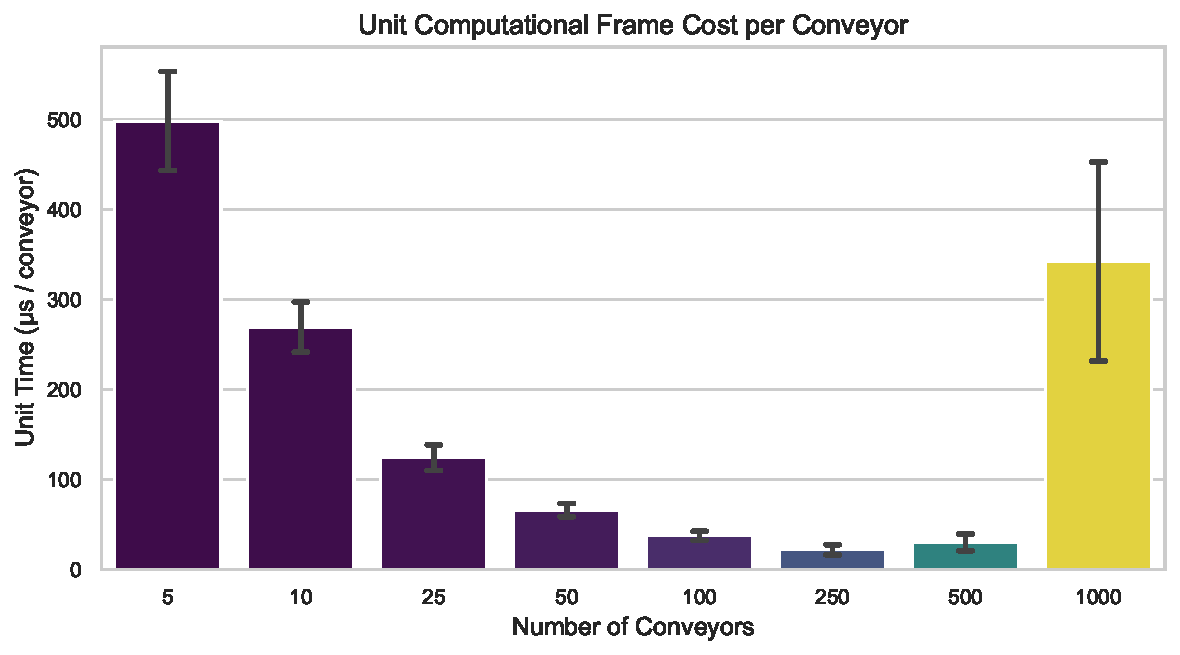
\includegraphics[width=0.88\linewidth,height=0.40\textheight,keepaspectratio]{5-Figures/eval_unit_frame_cost.pdf}
    \caption{Unit computational processing cost per conveyor module in microseconds ($\mu$s/conveyor).}
    \label{fig:eval_unit_frame_cost}
\end{figure}

As shown in \Cref{fig:eval_unit_frame_cost}, the unit computational cost per conveyor module reveals an inverse scaling efficiency at moderate counts. Processing an individual conveyor requires approximately 498\,$\mu$s at $N=5$, decreasing to 66\,$\mu$s at $N=50$, and reaching an optimal minimum of 21.7\,$\mu$s at $N=250$. Similar to the startup latency behavior, this inverse curve at low module counts is caused by Unity's fixed per-frame baseline engine work (such as main-thread loop orchestration, input polling, and graphics draw call setup), which is initially distributed across only a few conveyors. Once the layout scales to 50 and 250 modules, the engine operates with maximal efficiency before inter-collider matrix checks and physics contacts cause unit costs to rise sharply to 342.2\,$\mu$s per module at $N=1000$.

\subsection{Dynamic Temporal Stability and Statistical Correlations}
\label{sec:eval_timeseries_stability}

To verify that the simulation maintains stable behavior over extended operation without progressive frame degradation, \Cref{fig:eval_timeseries_fps} illustrates the dynamic \gls{FPS} time-series recorded across the benchmark execution window. \Cref{fig:eval_correlation_matrix} presents the Pearson linear correlation matrix computed across all recorded performance variables.

\begin{figure}[htbp]
    \centering
    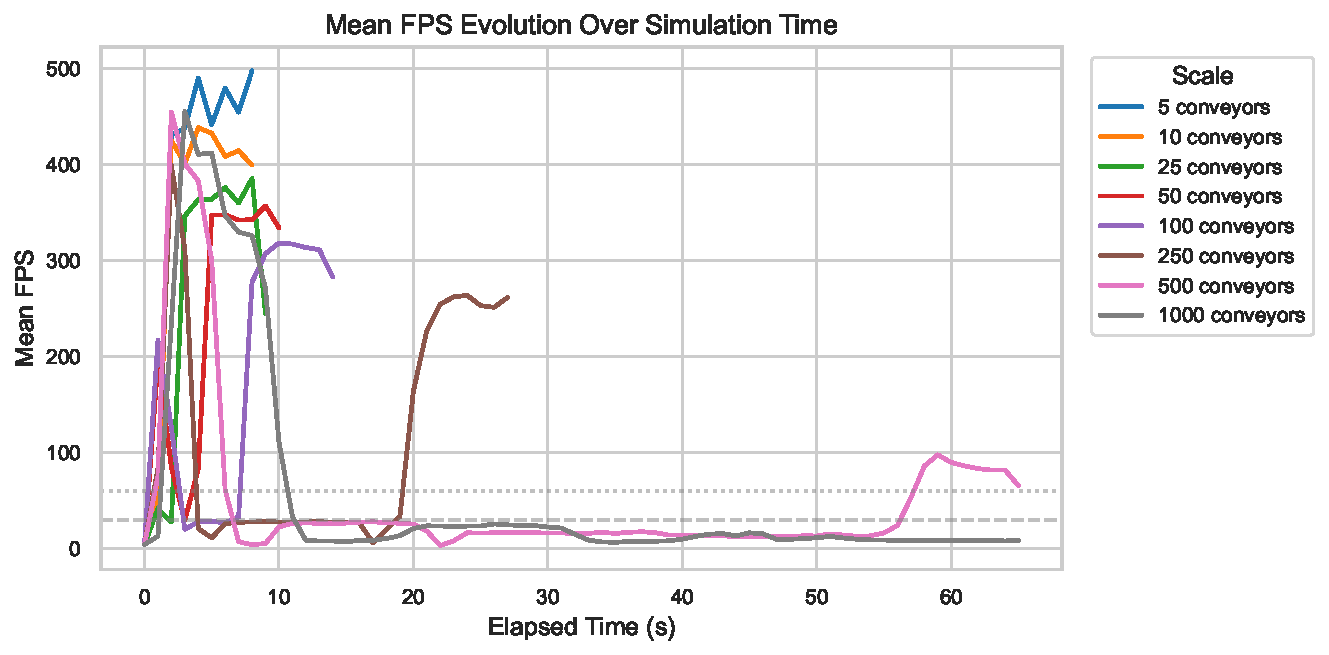
\includegraphics[width=0.90\linewidth,height=0.40\textheight,keepaspectratio]{5-Figures/eval_timeseries_fps.pdf}
    \caption{Dynamic simulation fluidity over the benchmark execution window across all evaluated module counts.}
    \label{fig:eval_timeseries_fps}
\end{figure}

The temporal profiles in \Cref{fig:eval_timeseries_fps} demonstrate clear phase separation. During the initial seconds of each run (corresponding to the startup times identified in \Cref{sec:eval_startup_complexity}), frame rates exhibit transient dips as assets are instantiated into the scene. Once initialization completes, all configurations from 5 to 250 conveyors enter steady-state execution, maintaining flat, stable frame rates across the entire measurement period.

\begin{figure}[htbp]
    \centering
    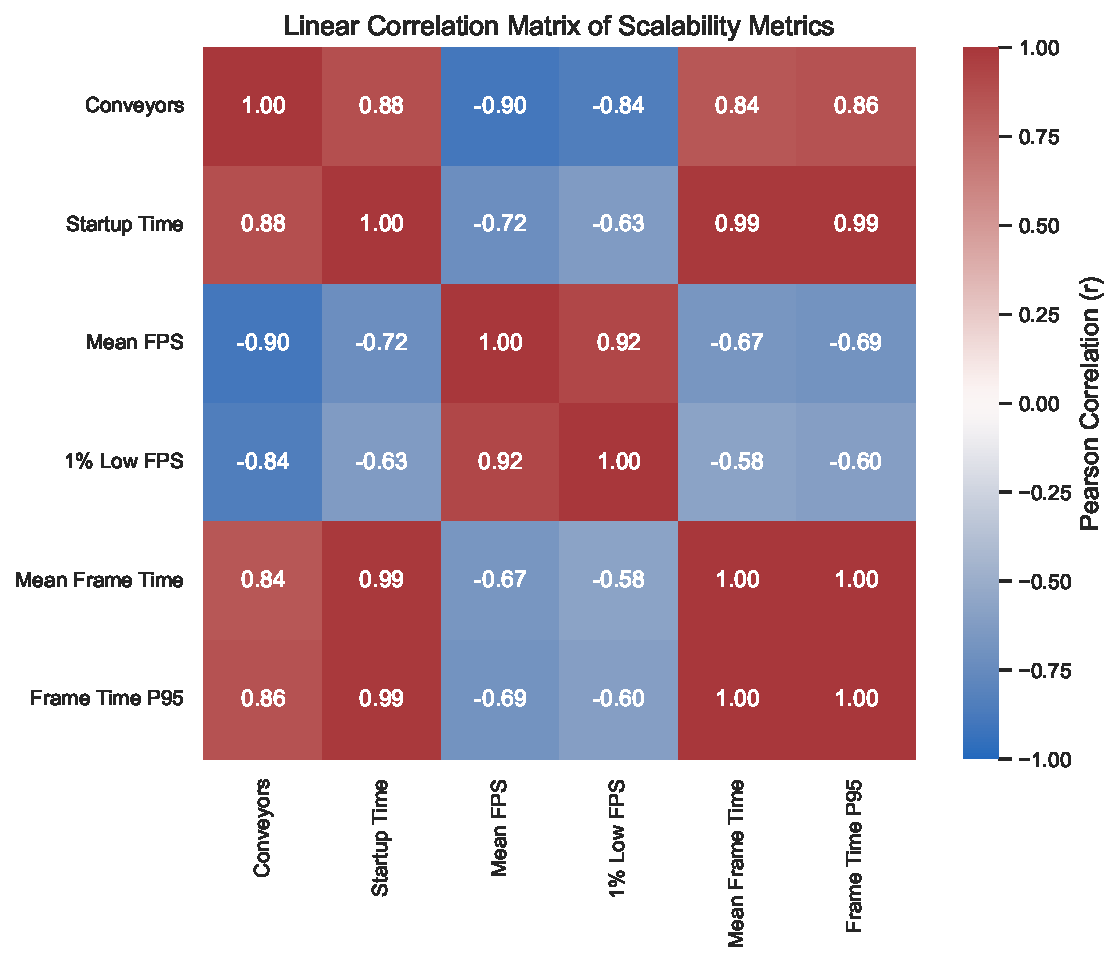
\includegraphics[width=0.88\linewidth,height=0.42\textheight,keepaspectratio]{5-Figures/eval_correlation_matrix.pdf}
    \caption{Pearson linear correlation matrix computed across procedural scalability metrics.}
    \label{fig:eval_correlation_matrix}
\end{figure}

The Pearson correlation matrix in \Cref{fig:eval_correlation_matrix} provides quantitative confirmation of key architectural behaviors:
\begin{itemize}
    \item \textbf{Conveyor Count vs.\ Frame Time ($r = 0.84$):} Computational frame latency correlates strongly with module count, demonstrating direct dependency on physics scene complexity.
    \item \textbf{Frame Time vs.\ Startup Time ($r = 0.99$):} Demonstrates that the processing overhead of mesh collider creation during startup directly mirrors the ongoing cost of narrow-phase collision checks during simulation.
    \item \textbf{Mean \gls{FPS} vs.\ 1\% Low \gls{FPS} ($r = 0.92$):} Confirms that frame drops remain tightly coupled to the underlying average performance rather than being triggered by anomalous background spikes.
\end{itemize}

\section{Discussion and Limitations}
\label{sec:eval_discussion}

The experimental results validate that the proposed framework can procedurally generate and execute industrial \gls{DT} simulations from standardized \gls{AAS} packages without pre-compiled scenes. Both the physical \gls{FMS} pilot bench validation and the high-density stress testing demonstrate key practical conclusions:

\begin{enumerate}
    \item \textbf{High-Fidelity Real-Time Feasibility:} For realistic modular production setups such as the \gls{FMS} bench, the \gls{DT} operates at nearly $490\,$\gls{FPS} with latencies of $2.36\,$ms, providing ample performance headroom to process bidirectional \gls{PLC} communication and physical synchronization without frame pacing issues. Across all realistic factory scales ($N \le 100$ conveyors), the runtime comfortably delivers over $300\,$\gls{FPS} and sub-$4\,$ms frame times, proving that real-world manufacturing cells operate with vast computational safety margins.
    \item \textbf{Single-Threaded Physics Bottleneck ($N > 500$):} Unity's default PhysX engine updates rigid-body dynamics sequentially on the main \gls{CPU} thread. While the framework scales comfortably up to 250 modules (averaging over 250\,\gls{FPS}) and maintains real-time execution at 500 modules (93\,\gls{FPS}), performance drops to 14\,\gls{FPS} at 1000 modules. For facilities exceeding 500 active conveyors, future work should implement spatial culling or migrate rigid-body dynamics to compute shaders using Unity's \gls{DOTS}.
    \item \textbf{Package Ingestion \gls{IO} Overhead:} At large scales, opening and extracting hundreds of separate \gls{AASX} zip archives introduces significant disk \gls{IO} overhead during startup ($416\,$s at 1000 modules). Implementing an in-memory package cache or pre-indexing submodel manifests could substantially reduce initialization times for large-scale production facilities.
    \item \textbf{Geometric Optimization Trade-Offs:} The fast loading times and low resource overhead observed in the benchmarks rely on the low-polygon geometric models generated in Layer~0. While these simplified meshes represent kinematic envelopes and sensor triggers accurately, they omit internal manufacturing details.
\end{enumerate}

\subsection{Systematic Verification of Research Objectives}

The empirical findings from both evaluation tracks directly validate the core research objectives formulated in \Cref{cha:introduction}:

\begin{itemize}
    \item \textbf{Semantic Asset Integration:} Confirmed. The modular \gls{AAS} submodel schema successfully united 3D visual geometry, kinematic bounds, virtual \gls{IO} pins, and declarative control rules. The exact same \gls{AASX} packages drove both standalone \gls{VC} in Unity and live physical hardware telemetry without modifying asset manifests.
    \item \textbf{Procedural Scene Assembly:} Confirmed. The runtime engine dynamically assembled all visual meshes, physical colliders, and telemetry bindings entirely in memory at launch (cold-boot initialization in $2.79 \pm 0.04\,$s for the pilot bench and $5.22 \pm 0.09\,$s for a 50-conveyor layout), fully eliminating pre-compiled scenes.
    \item \textbf{Real-Time Synchronization and Scalability:} Confirmed. Decoupling the asynchronous \gls{TCP} telemetry stream from the fixed physics loop alongside sensor-triggered kinematic snapping maintained continuous physical-digital alignment without drift. Parametric stress testing mapped the deterministic operational ceiling up to 500 modules ($93\,$\gls{FPS}) and isolated the single-threaded \gls{CPU} physics saturation at $N=1000$.
\end{itemize}

Overall, the evaluation demonstrates that the framework provides responsive, bounded real-time performance for modular production lines containing up to 250 modules, while maintaining valid operational fidelity up to 500 modules, confirming the feasibility of procedural \gls{DT} generation in smart manufacturing.